\documentclass{article}

% Language setting
% Replace `english' with e.g. `spanish' to change the document language
\usepackage[french]{babel}

% Set page size and margins
% Replace `letterpaper' with `a4paper' for UK/EU standard size
\usepackage[letterpaper,top=2cm,bottom=2cm,left=3cm,right=3cm,marginparwidth=1.75cm]{geometry}

% Useful packages
\usepackage{amsmath}
\usepackage{graphicx}
\usepackage[colorlinks=true, allcolors=blue]{hyperref}

\title{TP6 - Shadow Mapping}
\author{Beldjilali Maxime}

\begin{document}
\maketitle

\section{Lumières}

\subsection{Original}

\begin{figure}[h]
    \centering
    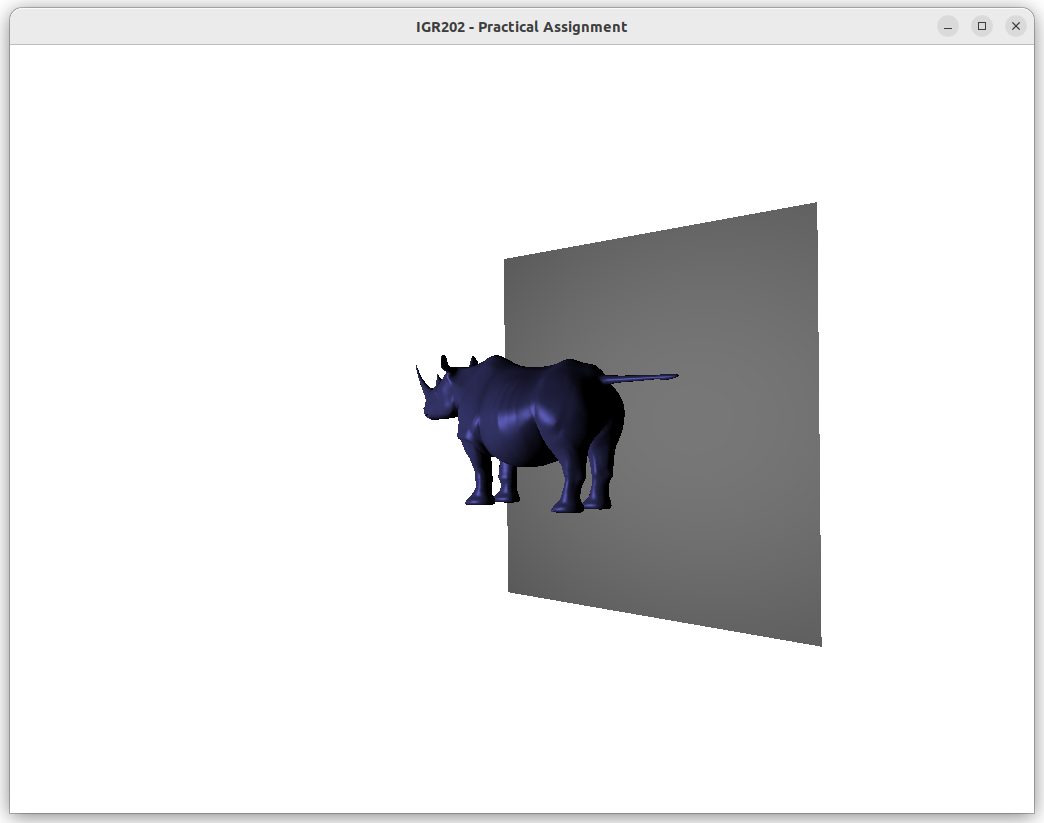
\includegraphics[width=0.5\linewidth]{images/oneLight.png}
    \caption{Original}
    \label{fig:original}
\end{figure}

\subsection{Trois sources lumineuses}

\begin{figure}[h]
    \centering
    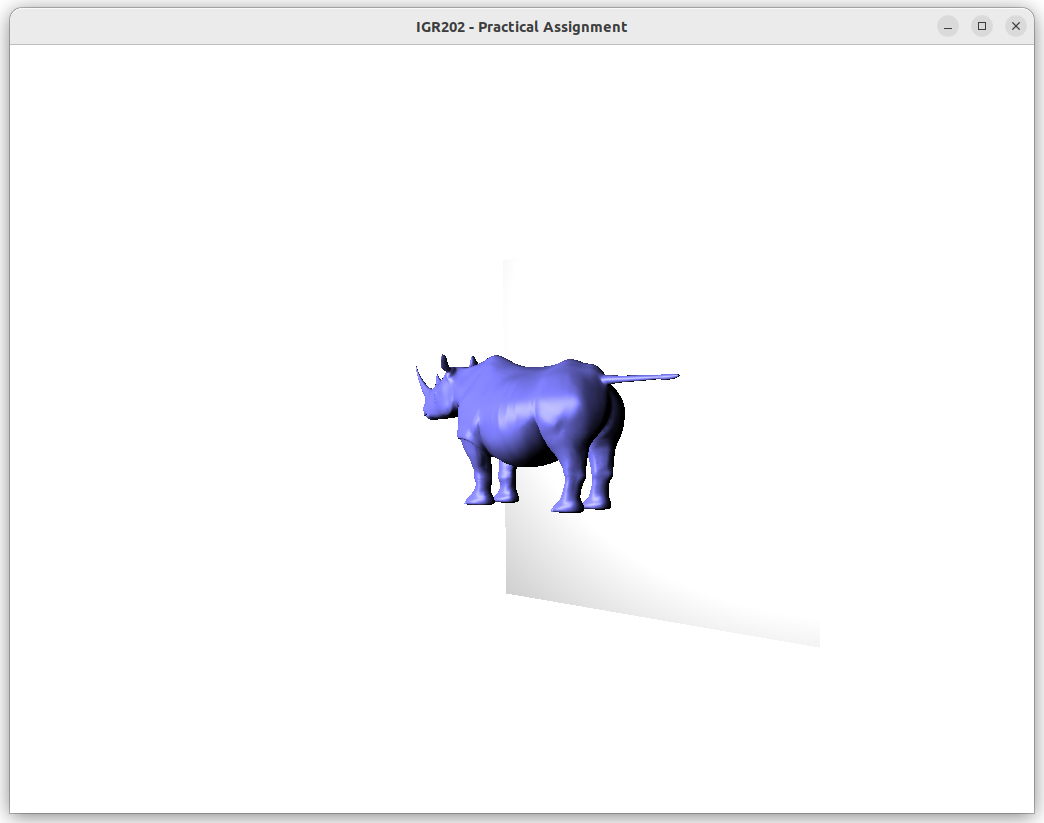
\includegraphics[width=0.5\linewidth]{images/threeLights.png}
    \caption{Trois sources lumineuses}
    \label{fig:threeLights}
\end{figure}

\section{Shadow Map}

\begin{figure}[h]
    \centering
    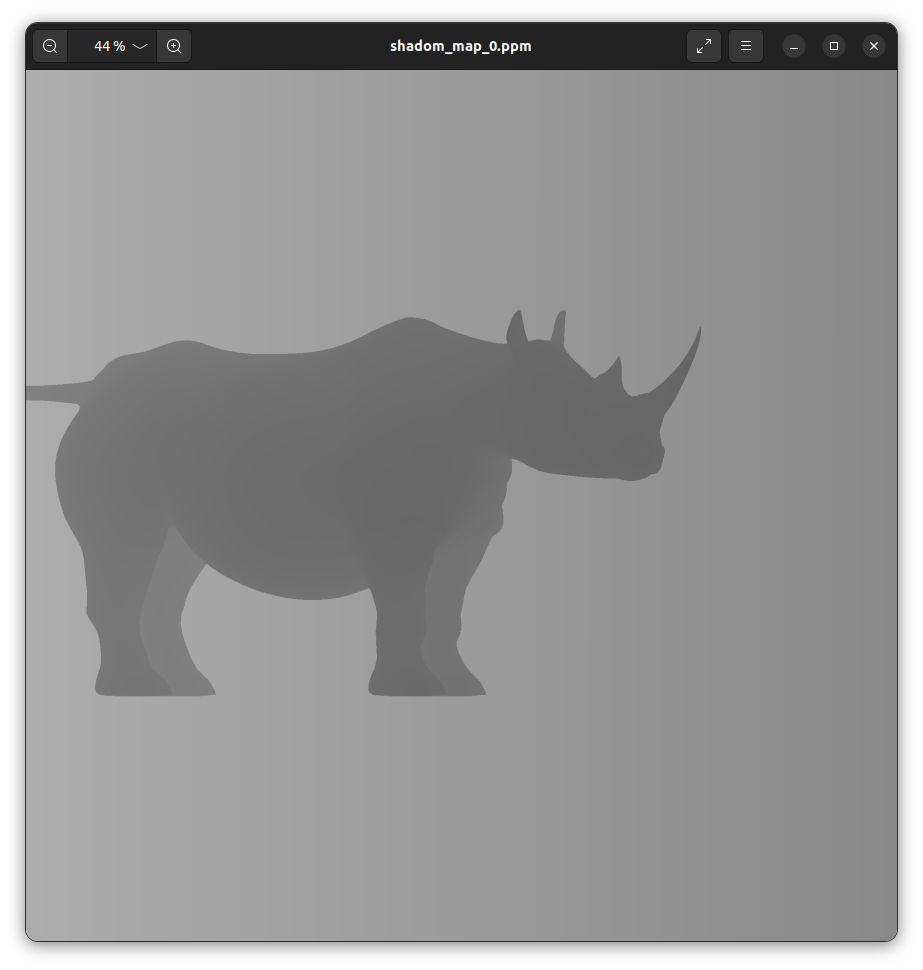
\includegraphics[width=0.5\linewidth]{images/depthMap.png}
    \caption{Shadow Map d'une source lumineuse}
    \label{fig:depthMap}
\end{figure}

\leavevmode
\newline


\section{Rendu des ombres}

\subsection{Rendu brute}

\begin{figure}[h]
    \centering
    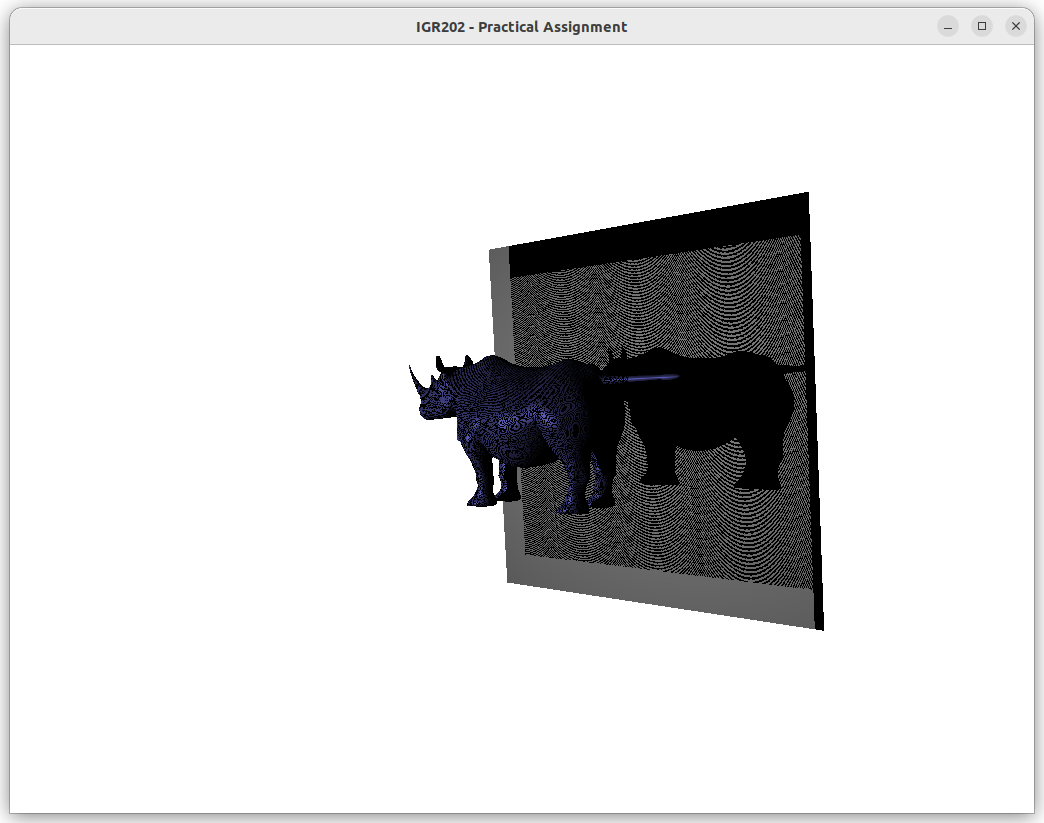
\includegraphics[width=0.5\linewidth]{images/raw.png}
    \caption{Rendu brute}
    \label{fig:raw}
\end{figure}

\newpage

\subsection{Avec un biais}

On ajoute un biais afin d'éviter l'artéfact d'auto-ombrage.
On fait en sorte que notre biais dépende de l'angle entre la normal et la direction de la lumière.
\[
    bias = max(0,05 \times (1 - \langle \Vec{N} \cdot \Vec{L} \rangle),\ 0.005) 
\]

\begin{figure}[h]
    \centering
    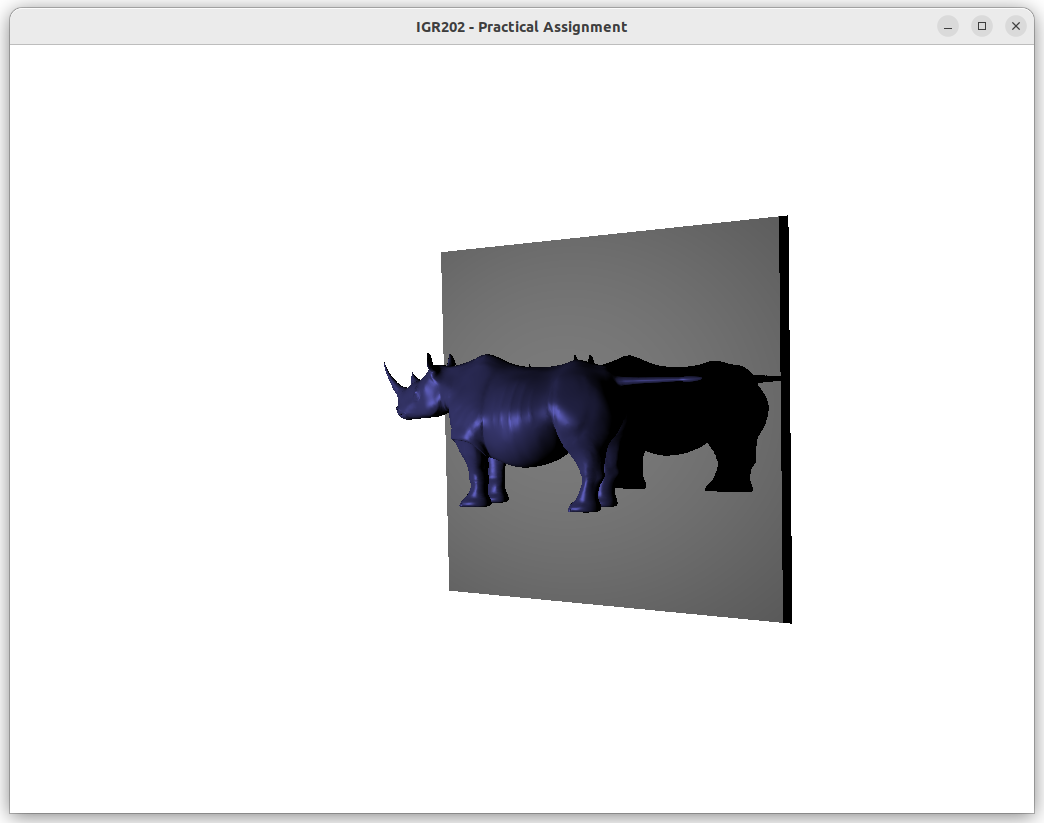
\includegraphics[width=0.5\linewidth]{images/bias.png}
    \caption{Avec biais}
    \label{fig:bias}
\end{figure}

\subsection{Avec face culling}

On obtient un décalage en rajoutant un biais. On peut éviter ce décalage en changeant le mode de face culling au moment du calcul de la depth map.

\begin{figure}[h]
    \centering
    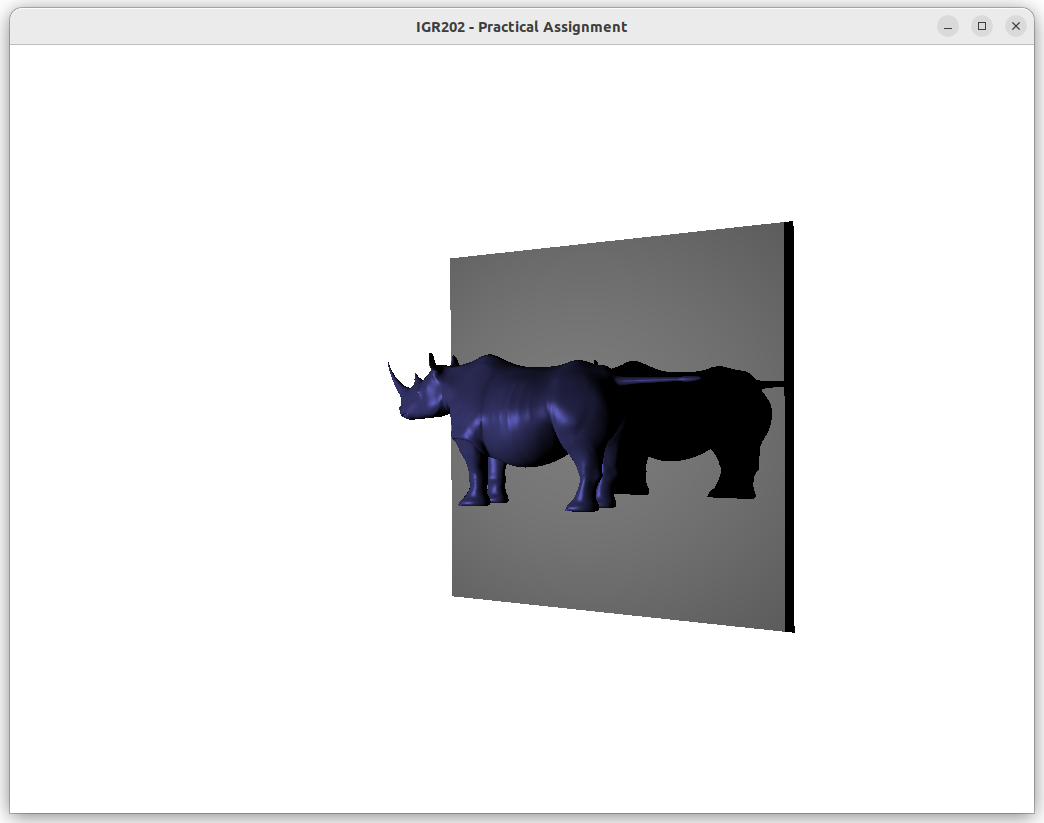
\includegraphics[width=0.5\linewidth]{images/cullFace.png}
    \caption{Juste avec le front-face culling}
    \label{fig:cullFace}
\end{figure}

\newpage

\subsection{Avec biais et front-face culling}

\begin{figure}[h]
    \centering
    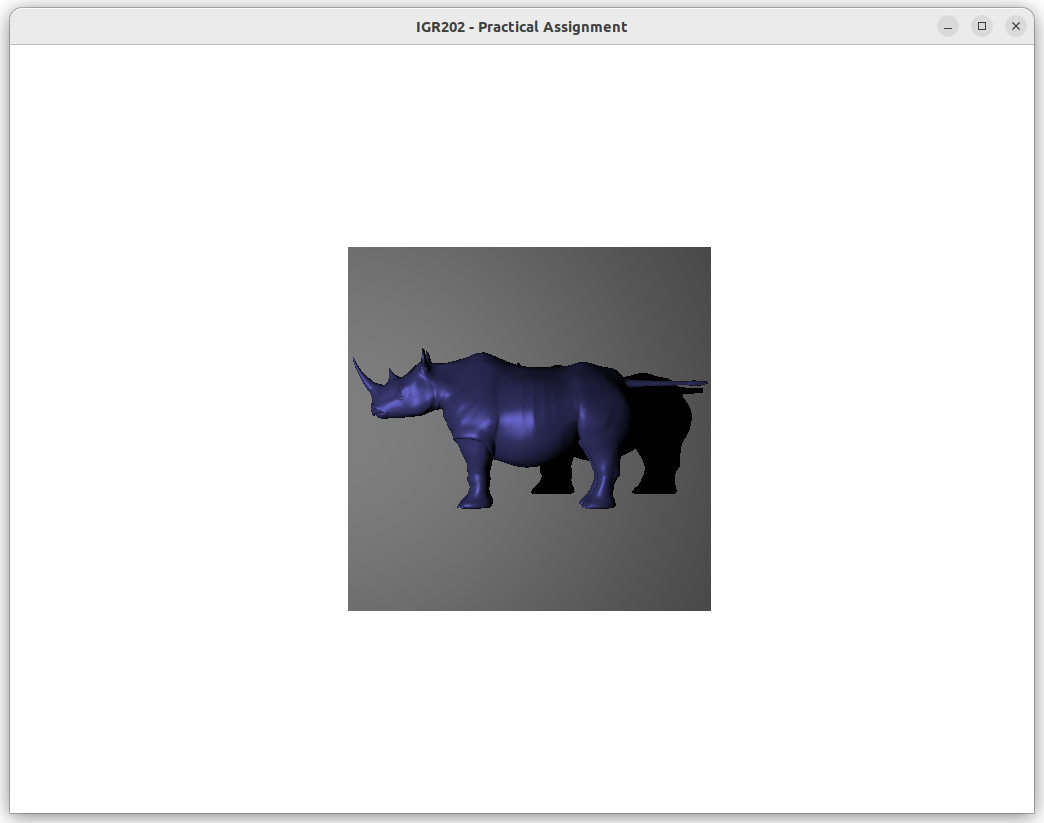
\includegraphics[width=0.48\linewidth]{images/cullFaceEtBias-1.png}
    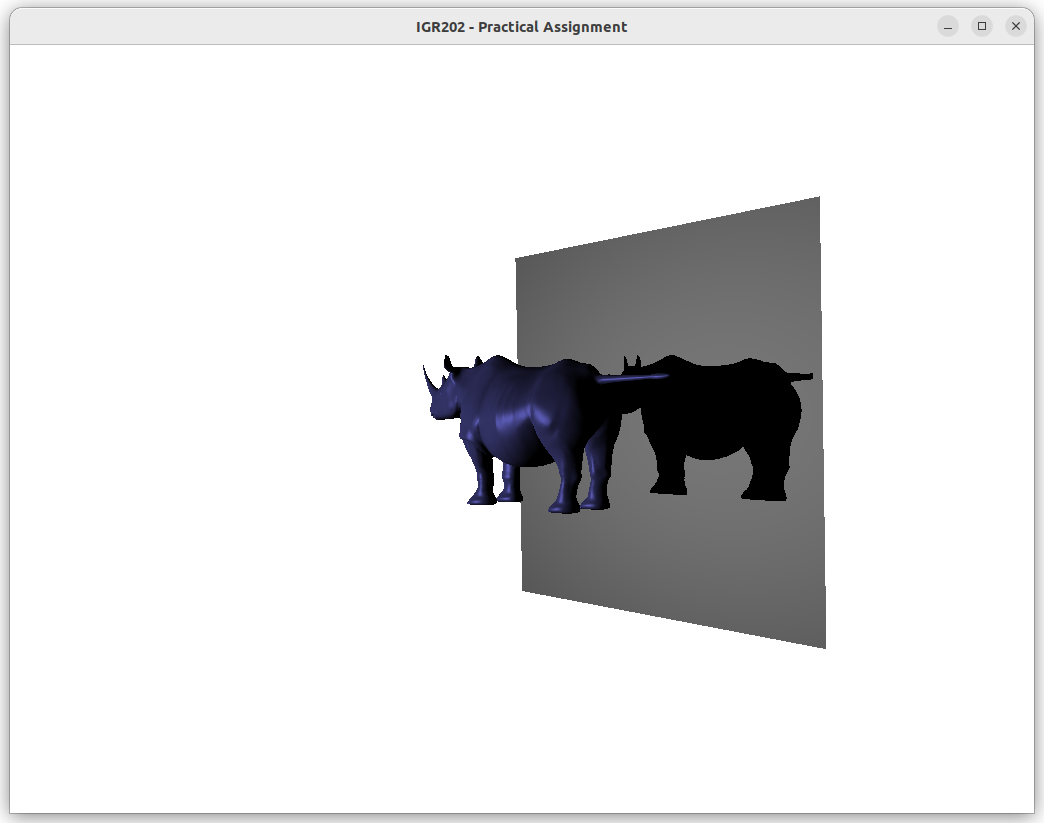
\includegraphics[width=0.48\linewidth]{images/cullFaceEtBias-2.png}
    \caption{Avec biais et front-face culling}
    \label{fig:cullFaceEtBias}
\end{figure}

\section{Avec trois sources lumineuses, biais et front-face culling}

\begin{figure}[h]
    \centering
    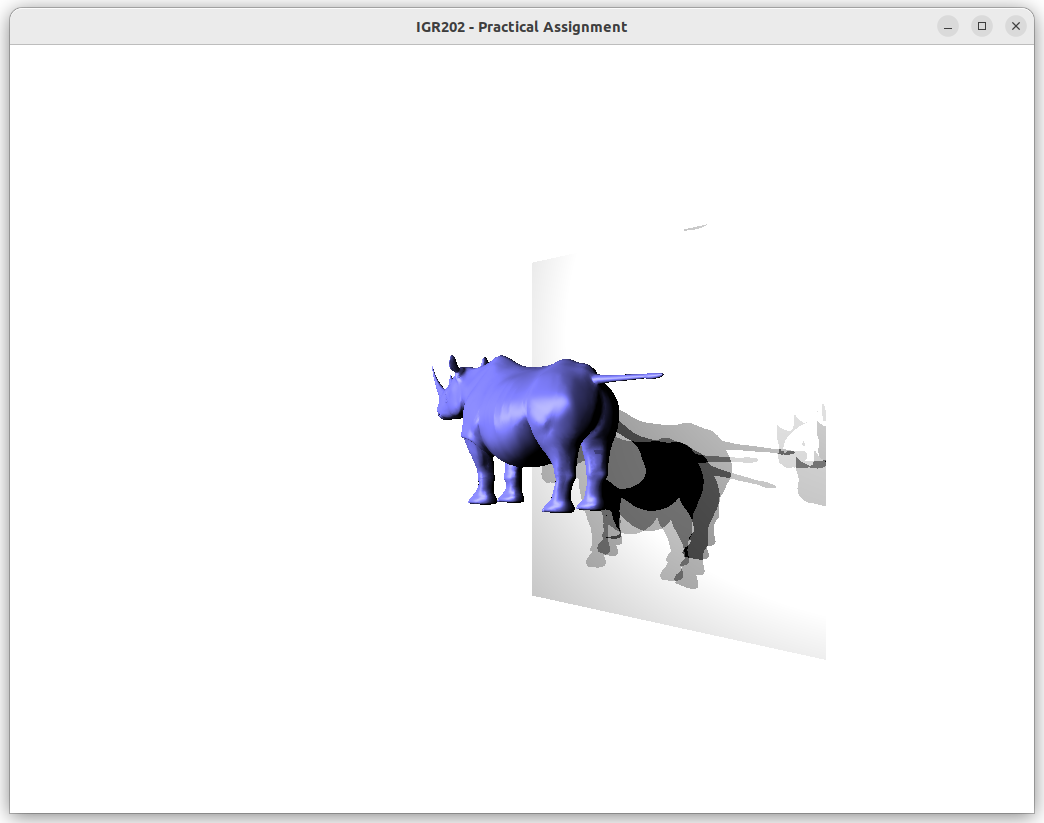
\includegraphics[width=0.5\linewidth]{images/cullFaceEtBiasMultipleLights.png}
    \caption{3 sources lumineuses + biais + front-face culling}
    \label{fig:cullFaceEtBiasMultipleLights}
\end{figure}

\section{Annexe}

Pour build :
\begin{enumerate}
    \item Ouvrir un terminal dans /BaseGL
    \item 
        \begin{verbatim}
mkdir build && cd build && cmake .. && cd .. && cmake --build build
        \end{verbatim}
\end{enumerate}

Pour lancer :
\begin{enumerate}
    \item Ouvrir un terminal dans /BaseGL
    \item 
        \begin{verbatim}
cmake --build build/ && ./BaseGL
        \end{verbatim} 
\end{enumerate}

\end{document}